\documentclass[Main.tex]{subfiles}
\begin{document}
\section{Experimenten en resultaten}
Voor het verder verklaren van de experimenten zijn er een aantal zaken die vermeld moeten worden. De volgorde waarin de experimenen zijn uitgevoerd is van belang. Bij de meeste experimenten wordt er gebaseerd op de resultaten van de voorgaande experimenten. Er zijn verschillende beoordelingswijzen die gebruikt worden bij het onderzoeken van de experimenten. Enerzijds testen de experimenten op oplossingsgraad\footnotemark[\ref{note:oplossingsgraad}] en anderzijds op de tijdsmarge die het algoritme nodig heeft. 
\par
Indien er niet gebaseerd wordt op de resultaten van vorige experimenten, dan zijn sommige van de latere experimenten enorm tijdrovend. Deze tijdrovende experimenten tonen ook niets aan wat niet aangetoond kan worden met de huidige manier van experimenteren.
\par
Alle experimenten zijn uitgevoerd op een \textit{2.26 GHz Intel Core 2 Duo} processor. Elk experiment is uitgevoerd met 500 iteraties. Alle experimenten zijn uitgevoerd op een bewerkingsboom met diepte vijf, tenzij anders vermeld. Een bewerkingsboom van diepte vijf betekend dat vergelijkingingen zoals $A^{B}+C \div D \ast E$ gevonden kunnen worden maar $A^{B}+C \div D \ast E \ast A$ niet. Bij elk van deze iteratie worden er twee voorbeelden gegeven waaraan de vergelijking moet voldoen.


\subsection{Pruning in bewerkingsboom} \label{ssec:pruning}
Zoals aangehaald in sectie \ref{ssec:Prunen} kan prunen in de bewerkingsboom de zoekruimte enorm verkleinen. Vooral omdat een absoluut redundante knoop ervoor zorgt dat al zijn kinderen nutteloos zijn. Wanneer deze dus weggehaald wordt vallen alle kinderen ook weg. In dit experiment zal bekeken worden hoeveel knopen er nu juist kunnen gepruned worden.
In de op voorhand gegenereerde boom bestaat er de mogelijkheid om te prunen. Op experimentele wijze wordt nu onderzocht hoeveel knopen overbodig zijn in de bewerkingsboom. Hiervoor wordt er een vergelijking gemaakt tussen het aantal knopen van de originele boom en het aantal knopen in deze nieuwe boom.
\par Zoals weergegeven in figuur \ref{fig:pruningInBewerkingsboom} stagneerd de besparing rond de 35\%. Dit heeft als gevolg dat bij het uitwerken van de bewerkingsboom 35\% minder vergelijkingen zullen moeten doorlopen worden. Het prunen op zich vraagt natuurlijk ook tijd. Daarom is de optie om de boom op voorhand te berekenen bekeken. Uit korte experimenten bleek echter al snel dat het voordeel klein is op lage niveaus. De besparing ligt ongveer rond de 100ms. Omdat het prunen van de uitwerking \\moeilijker is in deze geprunede bewerkingsboom is er vervolgens geopteerd de boom niet op voorhand te berekenen.
\begin{figure}
\centering
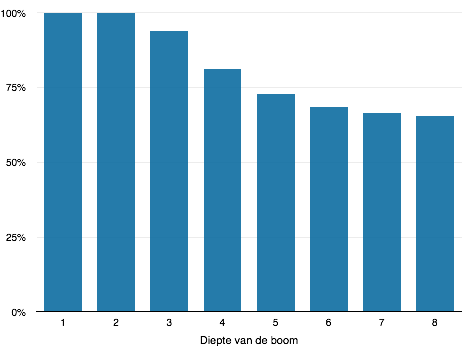
\includegraphics[width=\columnwidth]{treePrune.png} 
\caption{Resultaat pruning in bewerkingsboom.} \label{fig:pruningInBewerkingsboom}
\end{figure}

\subsection{Gewichten}
De volgende stap is het bepalen wat de invloed van het toevoegen van constanten heeft op de snelheid en de oplossingsgraad van het algoritme. In dit experiment worden er drie verschillende sets van waarden gebruikt, deze zijn $(1,2,3), (1,2,3,4,5)$ en $(1,2,3,5,7)$. De experimenten zijn uitgevoerd op een boom waar reeds de redundante knopen en bewerkingen (zie experiment \ref{ssec:pruning}) zijn uitgehaald. Om goed te kunnen vergelijken wordt zowel in figuur \ref{fig:gewichtenTijd} als in figuur \ref{fig:gewichtenOplossingsgraad} het resultaat getoond wanneer er geen constanten worden gebruikt. 
\par Wanneer we figuur \ref{fig:gewichtenTijd} en figuur \ref{fig:gewichtenOplossingsgraad} naast elkaar leggen, kan er besloten worden dat het gebruik van priemgetallen kleiner dan tien het beste resultaat opleverd. De grafieken spreken voor zich behalve wanneer het gebruik van de constanten $1, 2, 3, 4, 5$  naast het gebruik van de constanten $1, 2, 3, 5, 7$. De oplossingsgraad van deze tweede set van constanten ligt hoger simpelweg omdat met deze constanten makkelijker andere constanten gecombineerd kunnen worden door combinatie. De doorlooptijd bij het gebruik van de constanten $1, 2, 3, 4, 5$ ligt lager door de manier van prunen die wordt gebruikt. Het is namelijk niet toegelaten dat het combineren van constanten reeds bestaande constanten genereerd. Bij de set $1, 2, 3, 4, 5$ komt dit nu eenmaal vaker voor en dus worden er meer knopen gepruned waardoor er minder vergelijkingen moeten worden doorlopen.\par
Als algemene conclusie van dit experiment kan gesteld worden dat het gebruik van constanten weldegelijk een meerwaarde biedt. De zoektijd moet dan wel beperkt kunnen worden. De keuze van de set $1, 2, 3, 5, 7$ biedt de beste verhouding tussen verhoging van de oplossingsgraad en de vertraging. In de verdere experimenten zullen deze constanten dan ook gebruikt worden. Het is belangrijk om op te merken dat de mogelijkheid dat de gebruiker een voorbeeld geeft die deze waarden reeds bevat. Men moet echter beseffen dat bij een tweede voorbeeld deze waarden niet meer moet bevatten en dat de constanten dus wel degelijk nuttig blijven. Bovendien is er niet ge\"experimenteerd met constanten groter dan tien omdat niet verwacht wordt dat de gebruiker zulke vergelijkingen zoekt.

\begin{figure}[!htb]
\centering
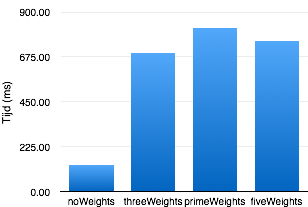
\includegraphics[width=\columnwidth]{weightsTijd.png} %TODO Tijden vergelijken
\caption{Vergelijking van de nodige tijd met het gebruik van constanten.} \label{fig:gewichtenTijd}
\end{figure}

\begin{figure}[!htb]
\centering
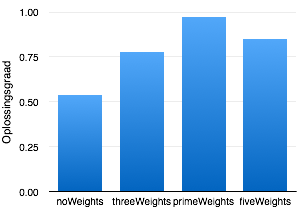
\includegraphics[width=\columnwidth]{weigthsSol.png} %TODO Oplossingsgraad vergelijken
\caption{Vergelijking van de oplossingsgraad bij het gebruik van constanten.} \label{fig:gewichtenOplossingsgraad}
\end{figure}

\subsection{Brute force vs Optimaliseren}
In deze laatste sectie zal het brute force algoritme vergeleken worden met het geoptimaliseerde algoritme. Het geoptimaliseerde algoritme is het algoritme besproken in bijlage \ref{sec:algorimteBesprekeing}. In figuur \ref{fig:brutevsopttijd} wordt de tijd vergeleken. Enerzijds kan er waargenomen dat het geoptimaliseerde algoritme weldegelijk sneller de niveaus doorloopt. Naarmate er dieper wordt gezocht neemt dit tijdsverschil toe. Echter blijven beide algoritmes exponentieel toenemen in tijd. De oplossingsgraad van beide zijn ongeveer gelijk. Het geoptimaliseerde algoritme vindt in sommige gevallen betere oplossingen. Hiermee wordt bedoelt vergelijkingen die de gebruiker in hogere waarschijnlijkheid zoekt. Zo wordt er verwacht dat de gebruiker liever een vergelijking vindt waarbij weinig constanten worden gebruikt maar wel alle kolomwaarden. Desondanks neemt dit niet weg dat de resultaten niet positief zijn. Daarom is er gezocht naar een eventuele heuristiek om de zoekboom te doorlopen. Er werd geen heuristiek gevonden, dit komt door het feit dat de productieregels van de context vrije grammatica toelaten dat de resulaten van ouder en kind enorm verschillen.


\begin{figure}[!htb]
\centering
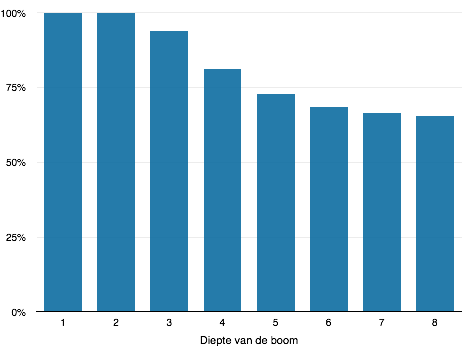
\includegraphics[width=\columnwidth]{treePrune.png} %TODO Tijden vergelijken
\caption{Vergelijking van de tijd die het brute force algoritme nodig heeft en die het geoptimalisseerde algoritme nodig heeft om 5 niveaus diep te berekenen.} \label{fig:brutevsopttijd}
\end{figure}

\end{document}